\documentclass[11pt]{article}
\usepackage{xltxtra}
\usepackage{xgreek}
\usepackage{mathtools}
\usepackage{amsthm}
\usepackage{amssymb}
\usepackage{unicode-math}
\usepackage{xkeyval}
\usepackage[%
a4paper,%
textwidth=16cm,
top=2cm,%
bottom=2cm,%
headheight=25pt,%
headsep=12pt,%
footskip=25pt]{geometry}%
\usepackage[greek]{alterqcm}
\usepackage{tikz}
\usepackage{tkz-tab}
%%%%%%%%%%%%%%%%%%%%%%%%%%%%%%%%%%%%%%%%%%%%%%%%%%%%%
\def\PP#1{\texttt{\char`\\#1}}
\setmainfont[Mapping=tex-text]{Arno Pro}
\setmathfont[Scale=MatchUppercase]{Asana Math}
\setmonofont[Scale=MatchLowercase]{Consolas}
%%%%%%%%%%%%%%%%%%%%%%%%%%%%%%%%%%%%%%%%%%%%%%%%%%%%%%%%%%%%%%%%%%



\begin{document}
	\title{Το πακέτο alterqcm. Δημιουργία καλαίσθητων διαγωνισμάτων με ερωτήσεις κλειστού τύπου.}
	\author{Απόστολος Συρόπουλος-Τάσσος Δήμου}
	\date{24 Ιουνίου 2019}
	\maketitle
\section{Εισαγωγή} 
Ο Alain Matthes μας έχει συνηθίσει σε ενδιαφέροντα πακέτα για το \LaTeX\ , που είναι μάλιστα πολύ σχετικά με τα δικά μας προγράμματα, το στυλ και το ύφος τους. Ένα τέτοιο παράδειγμα είναι και το \texttt{tkz-tab}, που παρουσιάστηκε πέρυσι στο \texttt{https://tassosdimou.gr/variation-table}.

Το πακέτο \textsf{alterqcm} είναι ακόμη ένα πακέτο του Alain Matthes για το \LaTeX\, που θα μας βοηθήσει στη κατασκευή καλαίσθητων διαγωνισμάτων με ερωτήσεις πολλαπλής επιλογής και σωστού-λάθους.

Το \textsf{alterqcm}  τροποποιήθηκε από τους Απόστολο Συρόπουλο και Τάσσο Δήμου έτσι, ώστε να προσαρμοστεί στα δεδομένα του ελληνικού εκπαιδευτικού συστήματος. 

 Το άρθρο αναπτύσσει με λεπτομέρειες και πολλά παραδείγματα τις δυνατότητες του \textsf{alterqcm}. Δίνει οδηγίες για τη χρήση του και στο τέλος  θα δοθούν μερικά παραδείγματα διαγωνισμάτων.

\section{Εγκατάσταση του πακέτου}	
Θα υποδείξουμε έναν απλό τρόπο εγκατάστασης του πακέτου. Δημιουργούμε ένα φάκελο, στον οποίο θα αποθηκευτούν όλα τα αρχεία, που θα επεξεργαστούμε, μελετώντας το \textsf{alterqcm}. Με άλλα λόγια, στον φάκελο αυτόν αποθηκεύουμε τα αρχεία \texttt{.tex}, τις εικόνες που θα χρησιμοποιηθούν και το αρχείο \texttt{alterqcm.sty}, που θα κατεβάσουμε από τη διεύθυνση \texttt{https://ctan.org/pkg/alterqcm?lang=en}. Το πακέτο θα φορτωθεί με την επιλογή \texttt{greek}, δηλαδή θα δώσουμε την εντολή:
\begin{verbatim}
\usepackage[greek]{alterqcm}
\end{verbatim}
Όλα τα αρχεία θα έχουν την κλασσική δομή των αρχείων \texttt{.tex}.

Στο πρώτο μέρος, το προοίμιο, θα τοποθετήσουμε τα: 
\begin{verbatim}
\documentclass[11pt,a4paper]{article}
\usepackage{xltxtra}
\usepackage{xgreek}
\usepackage{mathtools}
\usepackage{amsthm}
\usepackage{amssymb}
\usepackage{unicode-math}
\usepackage{xkeyval}
\usepackage{multirow,longtable}
\usepackage[greek]{alterqcm}
\usepackage{tikz}
\usepackage{tkz-tab}
%%%%%%%%%%%%%%%%%%%%%%%%%%%%%%%%%%%%%%%%%%%%%%%%%%%%%%%%%
\parindent=0pt
\setmainfont[Mapping=tex-text,Ligatures=Common]{Minion Pro}
\setmathfont[Scale=MatchUppercase]{Asana Math}
\end{verbatim}	
Αν τo διαγώνισμα δεν περιέχει μαθηματικές εξισώσεις ή σύμβολα, τότε αφαιρούμε από το προοίμιο τα πακέτα\linebreak  \texttt{mathtools,amsthm,amssymb}. 
Το κύριο σώμα του διαγωνίσματος περιέχεται ανάμεσα στα 
\begin{verbatim}
\begin{document}
................
\end{document}
\end{verbatim}	

\section{Το περιβάλλον \texttt{alterqcm} και η μακροεντολή \texttt{\PP AQquestion}}	
	
Το περιβάλλον \texttt{alterqcm} εισάγεται, όπως όλα τα περιβάλλοντα με:
\begin{verbatim}
\begin{alterqcm}
...............
\end{alterqcm}
\end{verbatim}	
Φυσικά δέχεται διάφορες παραμέτρους, που θα αναλύσουμε διεξοδικά και θα εφαρμόσουμε στα επόμενα με πολλά παραδείγματα. 

Μέσα στο περιβάλλον  εντάσσουμε και την μακροεντολή \verb|\AQquestion|, με την οποία εισάγουμε ερωτήσεις πολλαπλής επιλογής. Σημειωτέον ότι κι εδώ έχουμε διάφορες παραμέτρους, που θα δούμε στην πορεία. 

Ας προχωρήσουμε στο πρώτο μας παράδειγμα. 

\vspace{10pt}
\includegraphics[scale=]{shadows_box.pdf}
\begin{enumerate}
	\item Ξεκινάμε ένα καινούργιο αρχείο, που το ονομάζουμε \texttt{doc1} και το σώζουμε στο φάκελο που δημιουργήσαμε, έστω τον \texttt{myfolder}. Έτσι θα έχουμε μέσα στο φάκελο \texttt{myfolder} το αρχείο \texttt{doc1.tex}.
	\item Στο προοίμιο του αρχείου τυπώνουμε:
	\begin{verbatim}
	\documentclass[11pt,a4paper]{article}
	\usepackage{xltxtra}
	\usepackage{xgreek}
	\usepackage{amsmath,amssymb}
	\usepackage{xkeyval}
	\usepackage{multirow,longtable}
	\usepackage{alterqcm}
	\setmainfont[Mapping=tex-text,Ligatures=Common]{Minion Pro} 
	\parindent=0pt
	\end{verbatim}
	\item Στο σώμα του αρχείου τυπώνουμε:
	\begin{verbatim}
\begin{alterqcm}
\AQquestion{Ερώτηση}{%
{Επιλογή 1},
{Επιλογή 2},
{Επιλογή 3}}
\end{alterqcm}
\end{document}
\end{verbatim}
	\item 
Ας αποκρυπτογραφήσουμε τώρα ό,τι τυπώσαμε στο κυρίως σώμα του εγγράφου μας. Ανοίξαμε αντιστοίχως κλείσαμε το περιβάλλον \texttt{alterqcm} με
\begin{verbatim}
\begin{alterqcm}
...............
\end{alterqcm}  
\end{verbatim}	
Μέσα σε αυτό προσθέσαμε την εντολή \verb|\AQquestion|, που συντάσσεται ως εξής:

\verb|\AQquestion{η ερώτηση}{{επιλογή 1η},{επιλογή 2η},...,{επιλογή n}}|	
	
Εξάγουμε το εκτυπώσιμο pdf και θα πάρουμε:
\end{enumerate}
\begin{center}
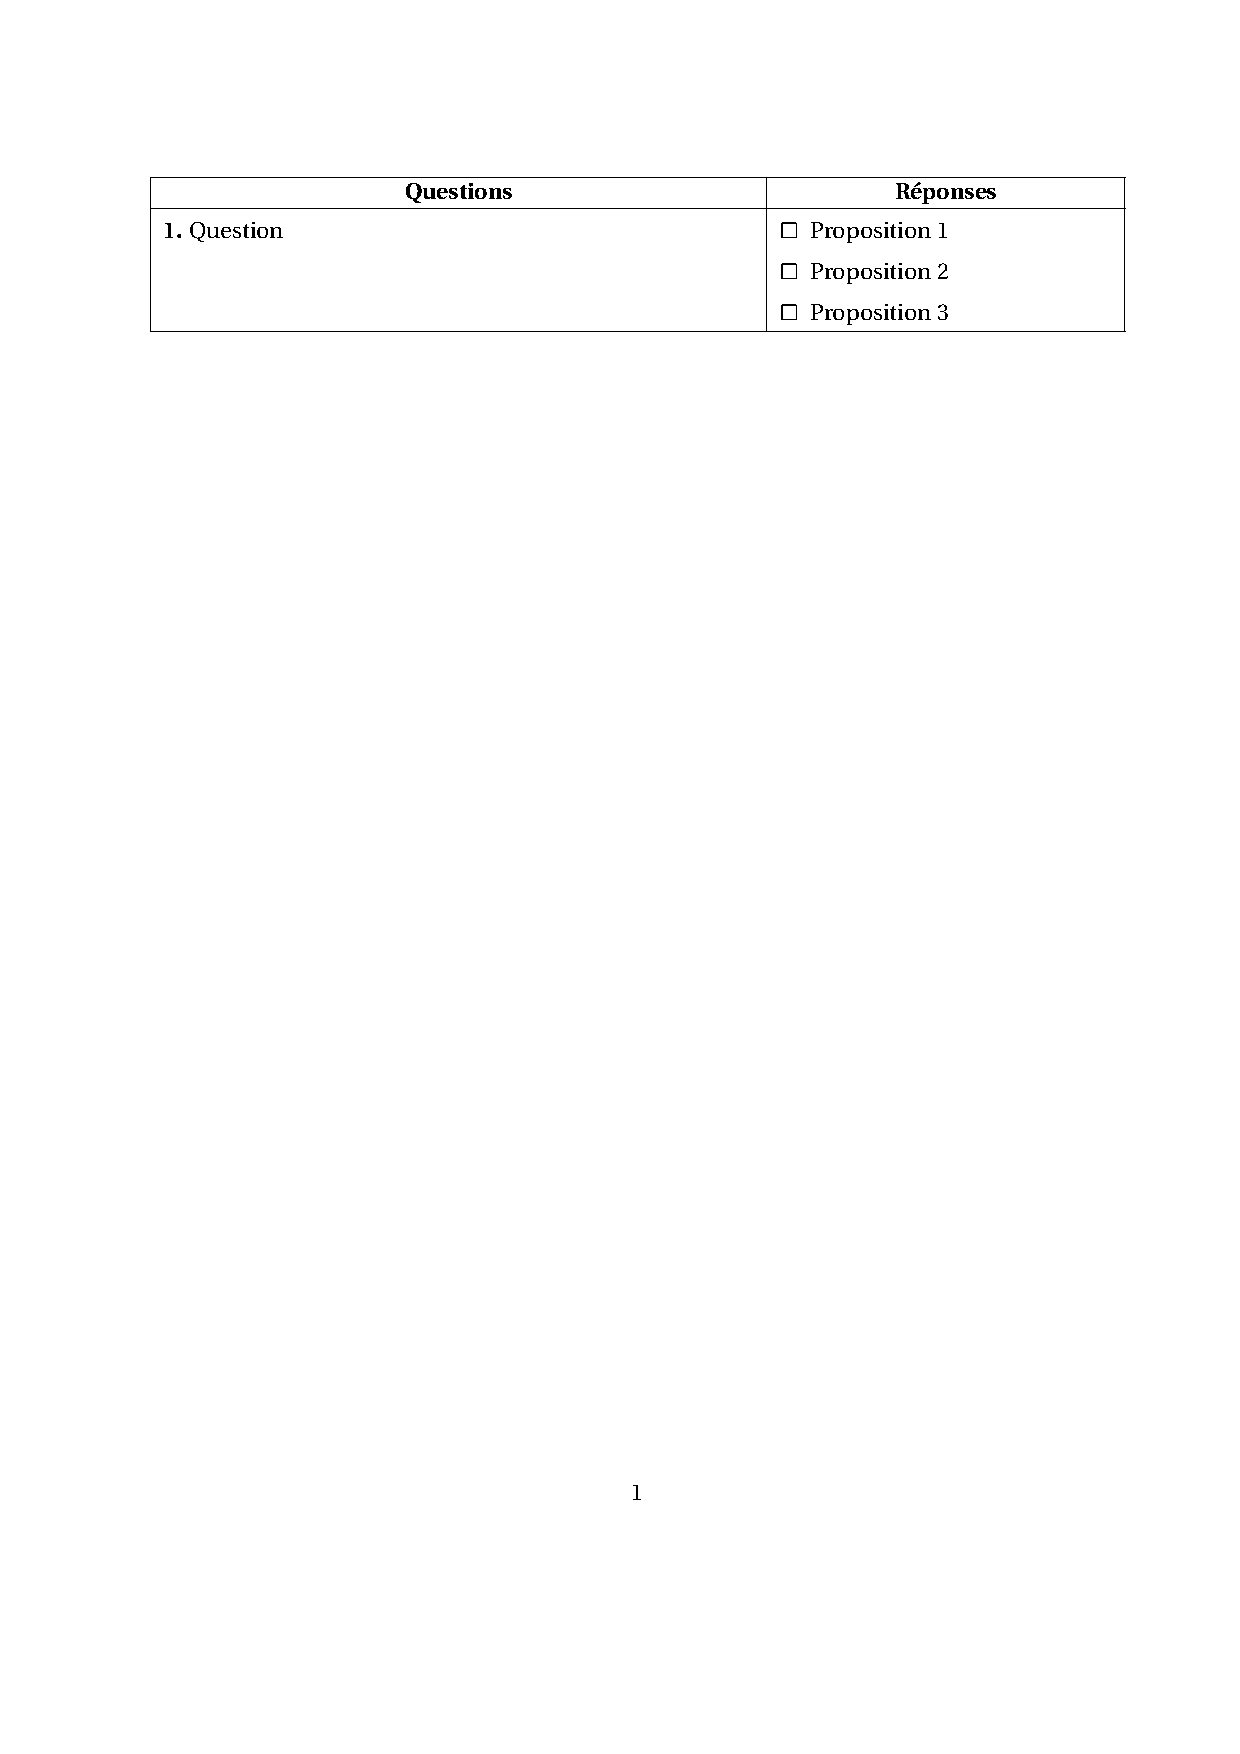
\includegraphics[scale=]{example_1.pdf}	
\end{center}

Όσες ερωτήσεις έχουμε, τόσες φορές με τον ίδιο τρόπο θα προσθέσουμε την εντολή \verb|\AQquestion|.

Στο παράδειγμά μας έγινε μια φορά.	

\subsection{Η παράμετρος \texttt{lq}}
Η παράμετρος \texttt{lq} ορίζει το πλάτος του κελιού της ερώτησης. Άρα έμμεσα ρυθμίζει και το πλάτος του πίνακα. Φυσικά σε κάθε περίπτωση έχουμε, αν απαιτείται, αναδίπλωση του κειμένου.
 Ας προχωρήσουμε σε ένα δεύτερο παράδειγμα.
\begin{center} 
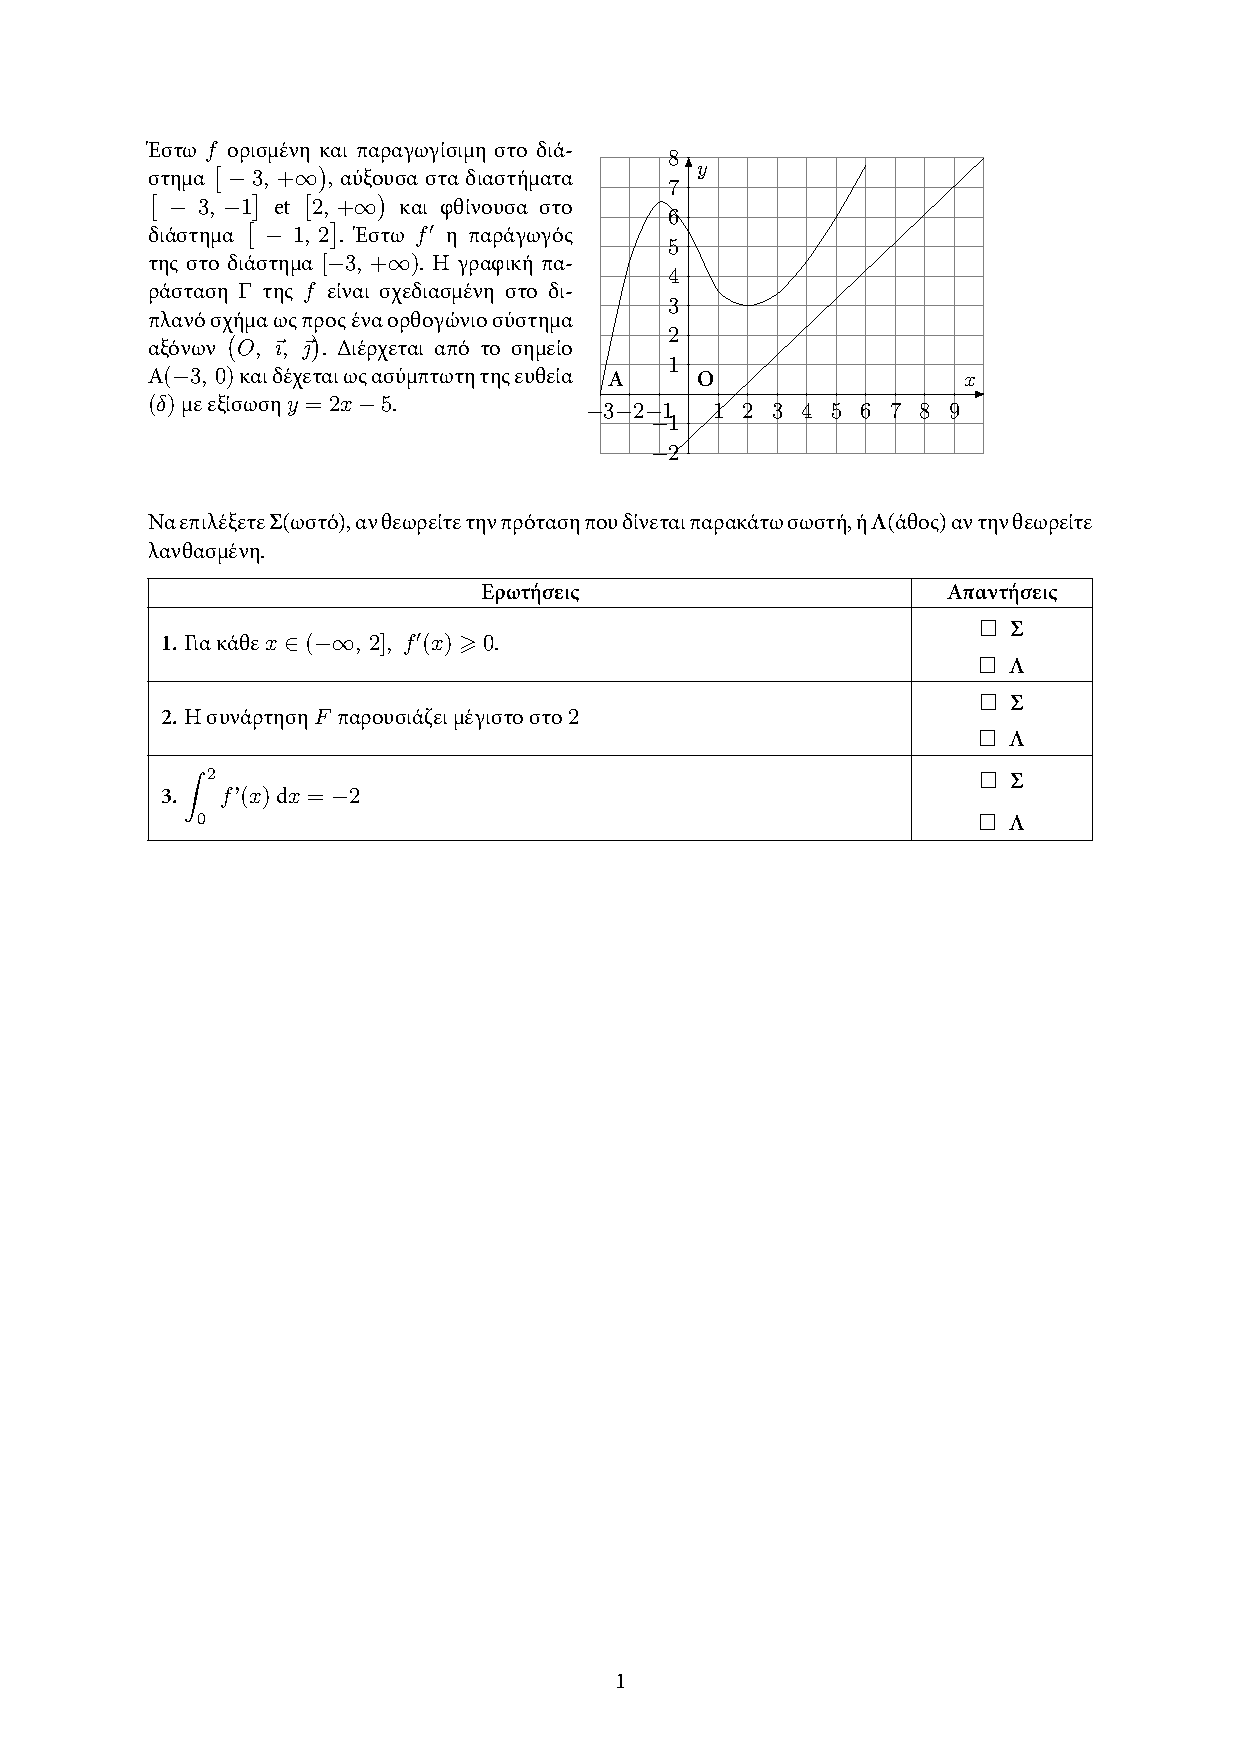
\includegraphics[scale=]{example_3.pdf} 
\end{center}
Για να πάρουμε το παραπάνω εκτυπώσιμο pdf, πληκτρολογήσαμε στο κυρίως σώμα του εγγράφου μας:  
\begin{verbatim}
\begin{alterqcm}[lq=5cm]
\AQquestion{Μεταξύ των διπλανών προτάσεων ποια είναι αυτή που αποδεικνύει ότι η 
  ασύμπτωτη της εκθετικής συνάρτησης έχει εξίσωση $y = 0$;}
{{$\displaystyle\lim_{x \to +\infty}\text{e}^x = + \infty$},
{$\displaystyle\lim_{x \to -\infty} \text{e}^x = 0$},
{$\displaystyle\lim_{x \to +\infty} \dfrac{\text{e}^x}{x} = + \infty$}}
\AQquestion[]{$e^{\ln x} = x$ για κάθε $x$ που ανήκει στο }
{{$\mathbf{R}$},
{$\big(0~;~+ \infty\big)$},
{$\big[0~;~+\infty\big)$}
}\end{alterqcm}
\end{verbatim} 
Εννοείται ότι το προοίμιο του αρχείου, παραμένει το ίδιο. Σώζουμε το αρχείο μας με το όνομα \texttt{doc2.tex} στο φάκελο \texttt{myfolder}. 
	
\section{Εφαρμογή του περιβάλλοντος \texttt{minipage}}
 	
Ας δούμε το προηγούμενο παράδειγμα ενταγμένο σε περιβάλλον \texttt{minipage}.
\begin{center}
\begin{minipage}{0.4\textwidth}
\begin{verbatim}
\begin{alterqcm}[lq=5cm]
\AQquestion{Μεταξύ των διπλανών
προτάσεων ποια είναι αυτή που
αποδεικνύει ότι η 
ασύμπτωτη της εκθετικής 
συνάρτησης έχει
 εξίσωση $y = 0$;}
{{$\displaystyle\lim_{x \to +\infty}
\text{e}^x = + \infty$},
{$\displaystyle\lim_{x \to -\infty}
\text{e}^x = 0$},
{$\displaystyle\lim_{x \to +\infty}
\dfrac{\text{e}^x}{x} = +\infty$}}
\AQquestion[]{$e^{\ln x} = x$ για 
κάθε $x$ που ανήκει στο }
{{$\mathbf{R}$},
{$\big(0~;~+ \infty\big)$},
{$\big[0~;~+\infty\big)$}
}\end{alterqcm}
\end{verbatim}
\end{minipage}
\begin{minipage}{0.5\textwidth}
\includegraphics[scale=0.63]{multiple_choice.pdf}
\end{minipage} 	
\end{center}
 	
\subsection{Η παράμετρος \texttt{pq}}	
	
Η παράμετρος \texttt{pq} ρυθμίζει την κάθετη απόσταση του κειμένου της ερώτησης από το πάνω μέρος του κελιού. Αν θέλουμε να έχει καθολική ισχύ (global), τότε την γράφουμε ως επιλογή του περιβάλλοντος \texttt{alterqcm}. Αν θέλουμε να ρυθμίσουμε μόνο μια ερώτηση, την προσθέτουμε ως παράμετρο της ερώτησης. Δηλαδή:

Για καθολική ισχύ (global): \verb|\begin{alterqcm}[lq=85mm,pq=2mm]|

Για τοπική ισχύ (local): \verb|\AQquestion[pq=2mm]|
\begin{center}
\includegraphics[scale=]{pq_global.pdf}	
\end{center}	
Για να έχουμε το παραπάνω αποτέλεσμα πληκτρολογήσαμε:
\begin{verbatim}
\begin{alterqcm}[lq=50mm,pq=2mm]
\AQquestion[pq=0mm]{Η ισότητα  $\ln (x^2 - 1) = \ln (x - 1) + \ln (x+1)$ είναι αληθής}
{{Για κάθε  $x\in (- \infty,\,-1) \cup(1,\,+ \infty)$}, {Για κάθε $x\in\mathbf{R} - \{-1,\,1\}$.},
{Για κάθε $x\in (1,\,+\infty)$}}
\AQquestion{Για κάθε πραγματικό $x$, ο αριθμός \[\dfrac{\text{e}^x - 1}
{\text{e}^x + 2}\hskip12pt \text{ισούται με:} \] }
{{$-\dfrac{1}{2}$},
{$\dfrac{\text{e}^{-x} - 1}{\text{e}^{-x} + 2}$},
{$\dfrac{1 - \text{e}^{-x}}{1 + 2\text{e}^{-x}}$}}
\AQquestion{Θέτουμε $I=\int_{\ln2}^{\ln3}\dfrac{1}{e^x-1}
\text{d}x,~J=\int_{\ln2}^{\ln3}\dfrac{e^x}{e^x-1}
\text{d}x$ τότε το $I-J$ ισούται με:}
{{$\ln{\dfrac{2}{3}}$},
{$\ln{\dfrac{3}{2}}$},	
{$\dfrac{3}{2}$}
}
\end{alterqcm}
\end{verbatim}	
Παρατηρούμε ότι ορίσαμε ως καθολική τιμή το \verb|pq=2mm|, ενώ τοπικά στην  πρώτη ερώτηση θέσαμε \verb|pq=0mm|	
	
\section{Ερωτήσεις Σωστού - Λάθους}	
	
Ερωτήσεις πολύ συνηθισμένες στα διαγωνίσματα και στις εξετάσεις στην Ελλάδα. Η εισαγωγή τους γίνεται με το γνωστό περιβάλλον:
\verb|\begin{minipage}[VF]|. Το πακέτο είναι σε γαλλική γλώσσα και Vrai σημαίνει αλήθεια (σωστό) ενώ Faux σημαίνει λάθος. Για να δούμε τι συμβαίνει όταν προσθέσουμε την παράμετρο \verb|VF|.	

\begin{center}	
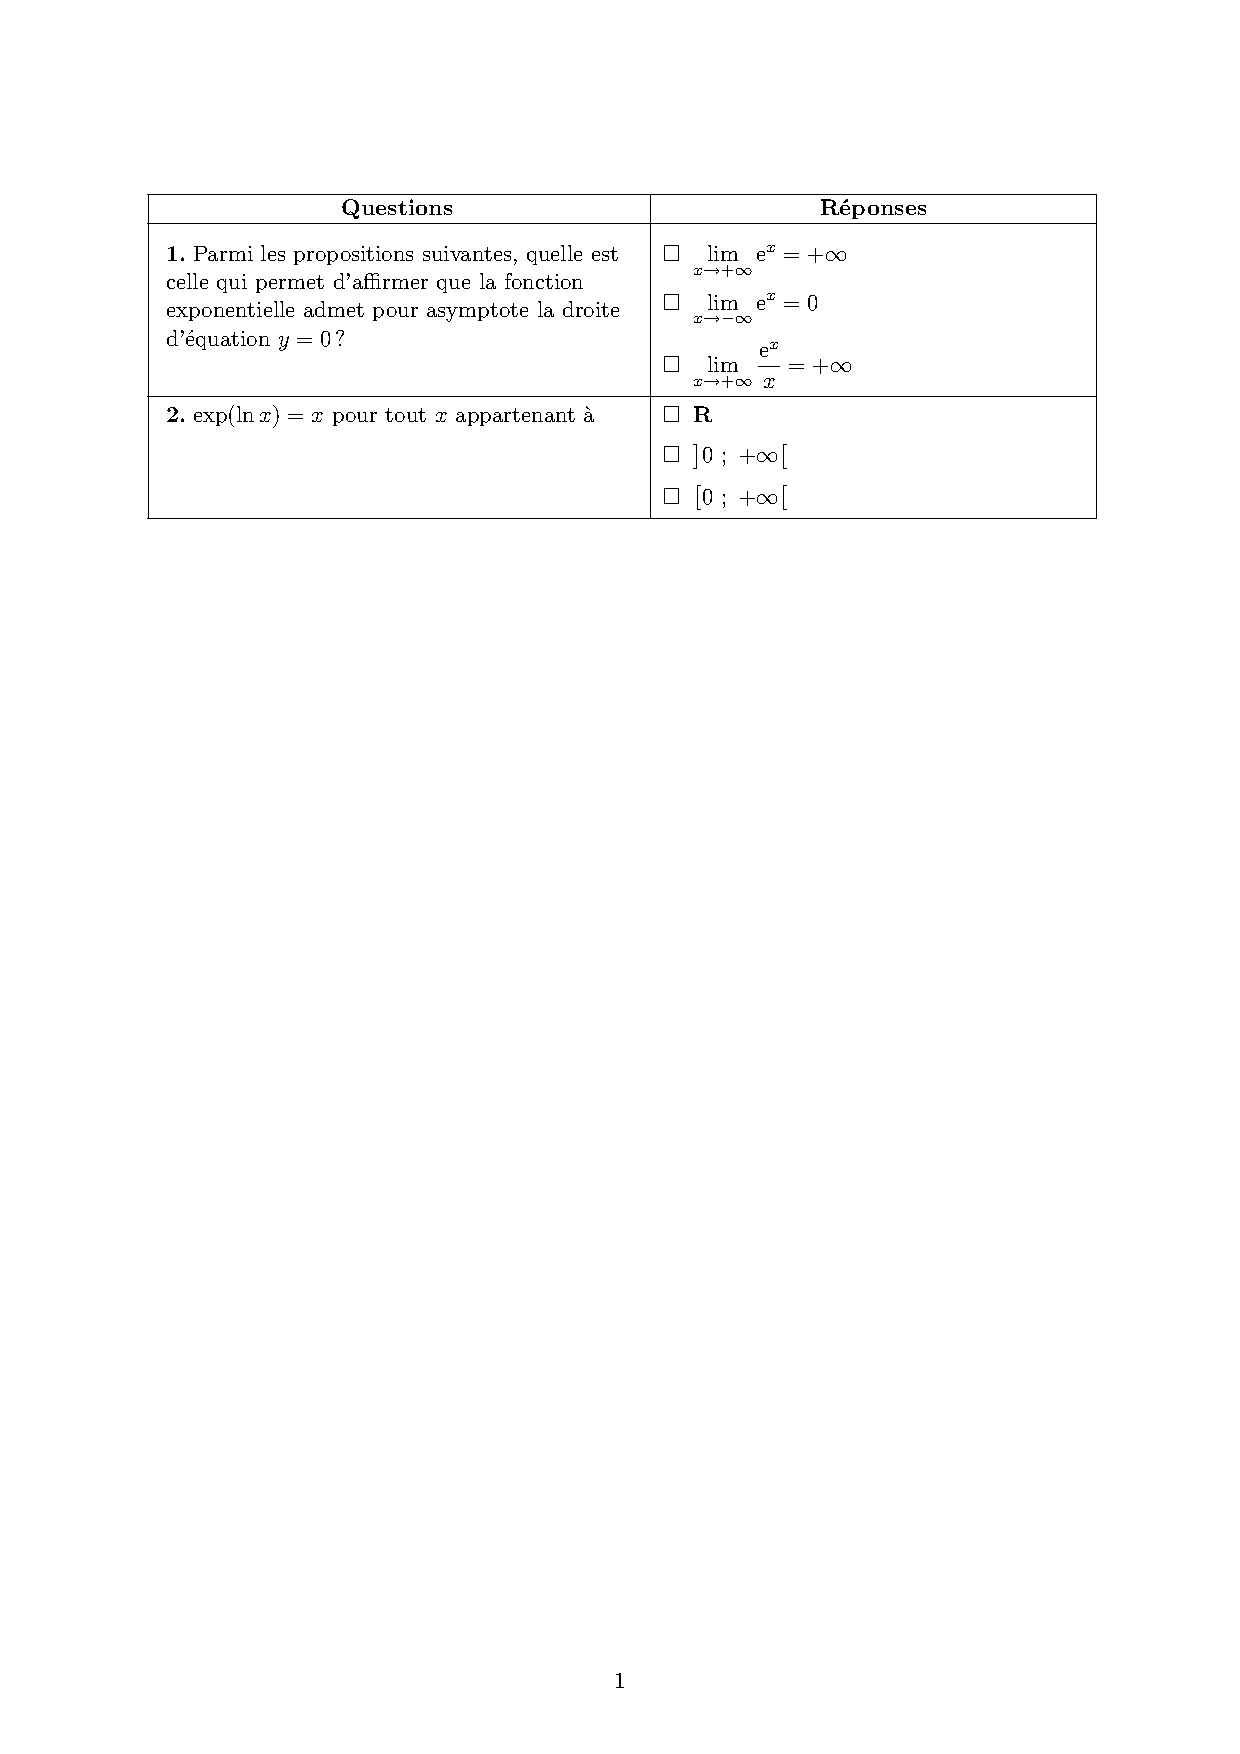
\includegraphics[scale=]{example_2.pdf}	
\end{center}
Ο κώδικας για το παραπάνω εκτυπώσιμο pdf είναι:
\begin{verbatim}
\begin{alterqcm}[VF,lq=60mm]
\AQquestion[]{Ισχύει ότι $(α+β)^2=α^2+β^2$}
\AQquestion[]{Αν $α\cdot β\geq 0$, τότε $\sqrt{α\cdot β}=\sqrt{α}\cdot\sqrt{β}$ }
\AQquestion[]{Είναι $|α|=α,\,\text{για κάθε}
 x\in\mathbb{R}$}
\end{alterqcm}
\end{verbatim}
\paragraph{Προσοχή}
Σχετικά με τα ελληνικά σε \emph{μαθηματικό περιβάλλον}. Στο \LaTeX\ τα ελληνικά εισάγονται με εντολές, όπως \verb|\alpha, \beta,κ.λ.π. \Alpha..|, αντίστοιχα για πεζά και κεφαλαία. Στο \XeLaTeX\ γράφουμε κανονικά τα ελληνικά, δηλαδή από το πληκτρολόγιο, αρκεί στο προοίμιο να έχουμε φορτώσει, εκτός από τα πακέτα \verb|xltxtra, xgreek|, επιπλέον το πακέτο \verb|unicode-math| και τη γραμματοσειρά \verb|Asana Math|, που δημιουργήθηκε και υποστηρίζεται από τον Απόστολο Συρόπουλο. Απλά δίνουμε την εντολή: 

\verb|\setmathfont[Scale=MatchUppercase]{Asana Math}|.  

\subsubsection*{Ένα πιο σύνθετο παράδειγμα Σωστού-Λάθους}
\begin{center}
\includegraphics[scale=0.95]{example_3_a_croped.pdf}
\end{center}
Στο παράδειγμα αυτό, παρουσιάζονται, κατά κάποιο τρόπο, δύο τμήματα. Στο πρώτο τμήμα, γράφουμε σε περιβάλλον \texttt{minimage} την εκφώνηση και παράλληλα το σχήμα (δημιουργήθηκε με χρήση του πακέτου tikz). Το δεύτερο τμήμα δημιουργήθηκε με το περιβάλλον \texttt{alterqcm} και έχει κώδικα:
\begin{verbatim}
\begin{alterqcm}[VF,pre=true,lq=125mm]
\AQquestion{Για κάθε $x \in (-\infty,\,2],
\;f^{\prime}(x) \geqslant 0$.}
\AQquestion{Η συνάρτηση $F$ παρουσιάζει
 μέγιστο στο $2$}
\AQquestion{$\displaystyle\int_{0}^2
 f^{\prime}(x)\:\text{d}x = - 2$}
\end{alterqcm}
 
\end{verbatim} 

\subsection{Η παράμετρος \texttt{pre}}

Η παράμετρος, αν πάρει τη τιμή  \texttt{pre=true} προσθέτει αυτόματα το κείμενο << Να επιλέξετε Σ(ωστό)...την απάντησή σας>>. Αυτό γίνεται όταν λειτουργεί μαζί με την παράμετρο \texttt{VF} στο όρισμα του περιβάλλοντος. Αν στο περιβάλλον δεν υπάρχει η \texttt{VF}, τότε η \texttt{pre=true} παράγει το κείμενο <<Για την ερώτηση που σας δίνεται,...την επιλογή σας>>, που παρουσιάζεται στις ερωτήσεις πολλαπλής επιλογής. Μπορούμε βέβαια να την αγνοήσουμε και να γράφουμε την "εκφώνηση", όπως την επιθυμούμε.

\subsection{Η παράμετρος \texttt{sep} }
Προσθέτοντας την παράμετρο \verb|\text=true| στο περιβάλλον \verb|alterqcm|, δημιουργούνται οριζόντιες γραμμές ανάμεσα στις επιλογές.

\vspace{15pt} 
\begin{minipage}{0.3\textwidth}
\begin{verbatim}
\nogreekalph 
\begin{alterqcm}
[lq=6cm,sep=true]
\AQquestion{Ερώτηση}
{{Πρόταση 1},
{Πρόταση 2},
{Πρόταση 3}}
\end{alterqcm}
\greekalph
\end{verbatim}
\end{minipage}
\begin{minipage}{0.6\textwidth}
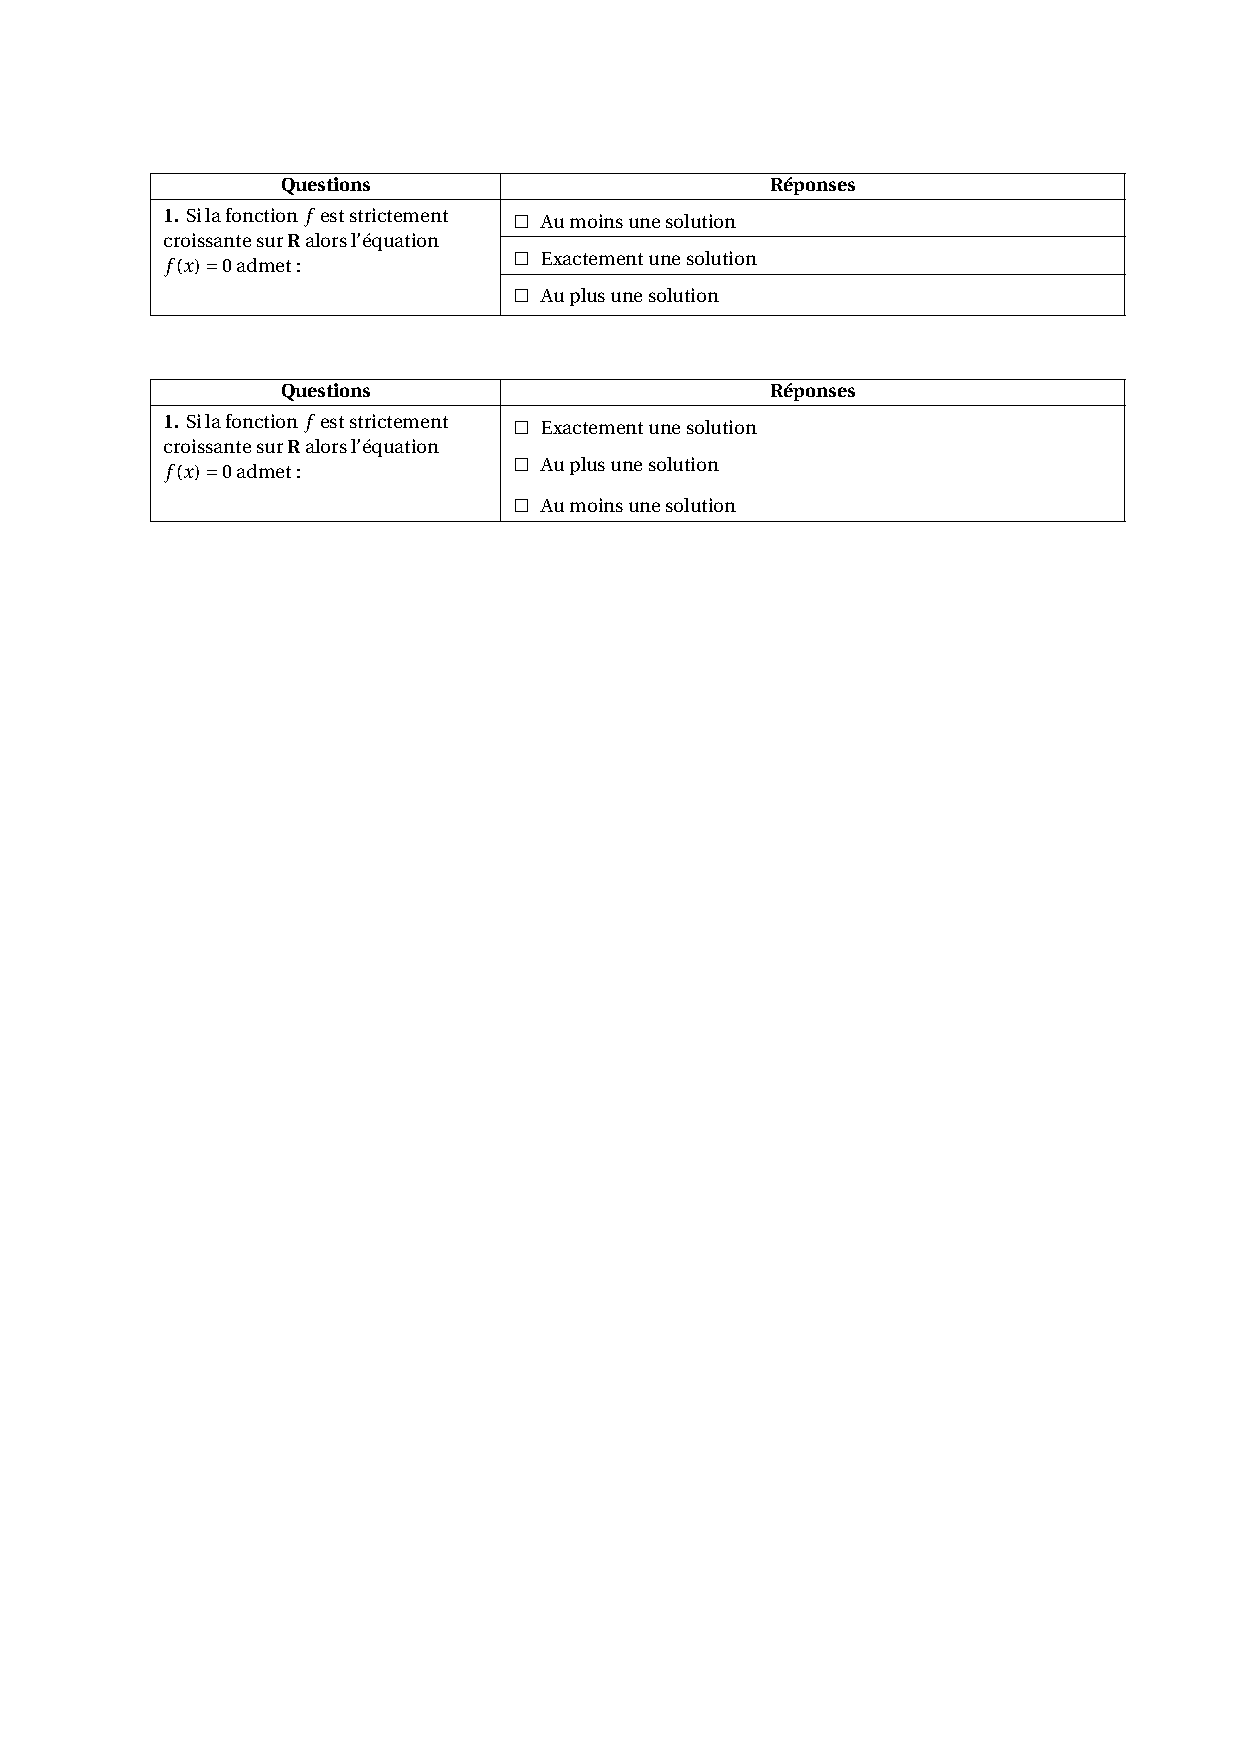
\includegraphics[scale=]{sep.pdf}
\end{minipage}

\subsection{Η παράμετρος \texttt{symb}}

Με την παράμετρο \texttt{symb} καθορίζουμε τη μορφή των τετραγώνων, που σημειώνονται οι απαντήσεις στα ερωτήματα. Οι τιμές που μπορεί να πάρει είναι \verb|\altersquare|, \verb|\dingsquare|, \verb|\dingchecksquare|. 

Για παράδειγμα, γράφουμε τον κώδικα:
\begin{verbatim}
\begin{alterqcm}
[VF,lq=125mm,pre=true, symb=\dingsquare]
\AQquestion{Οι ανισώσεις $2-\dfrac{x}{2}\leq
 x+\dfrac{1}{2}$ και $5x-5\geq 0$ έχουν 
 ίδιες λύσεις.}
\AQquestion{Ο αριθμός -2 είναι λύση της
 ανίσωσης $-2x+3<-5$.}
\AQquestion{Η ανίσωση $5x>-2$ είναι αδύνατη.}
\end{alterqcm}
\end{verbatim}
και θα πάρουμε σε εκτυπώσιμο pdf:
\begin{center}
\includegraphics[scale=0.95]{dingsquare_croped.pdf}
\end{center}
\subsection{Οι παράμετροι \texttt{num} και \texttt{numstyle}}

\subsubsection*{Η παράμετρος \texttt{num}}
Η παράμετρος \texttt{num} όταν παίρνει την τιμή \texttt{false}, δηλαδή \texttt{num=false} δεν εμφανίζει την αρίθμηση των ερωτήσεων. Αν \texttt{num=true}, τότε εμφανίζει την αρίθμηση. Για παράδειγμα:
\begin{center}
\begin{minipage}{0.4\textwidth}
\begin{verbatim}
\nogreekalph 
\begin{alterqcm}
[lq=3cm,num=false]
\AQquestion{Ερώτηση A}
{{Πρόταση 1},
{Πρόταση 2},
{Πρόταση 3}}
\AQquestion{Ερώτηση Β}
{{Πρόταση 1},
{Πρόταση 2},
{Πρόταση 3}}
\end{alterqcm}
\greekalph
\end{verbatim} 
\end{minipage}
\begin{minipage}{0.5\textwidth}
\includegraphics[scale=0.95]{num_false_a.pdf}
\end{minipage}
\end{center}

\subsection{Η παράμετρος \texttt{numstyle}}

Αν η παράμετρος \texttt{numstyle} πάρει την τιμή \verb|\alph|, δηλαδή \verb|numstyle=\alph|, τότε τροποποιείται το στυλ αρίθμησης των ερωτήσεων και παίρνει τη μορφή (a., b., c.,...). Για παράδειγμα:
\begin{center}
\begin{minipage}{0.4\textwidth}
\begin{verbatim}
\begin{alterqcm}
[lq=3cm,numstyle=\alph]
\AQquestion{Ερώτηση A}
{{Πρόταση 1},
{Πρόταση 2},
{Πρόταση 3}}
\AQquestion{Ερώτηση Β}
{{Πρόταση 1},
{Πρόταση 2},
{Πρόταση 3}}
\end{alterqcm}
\end{verbatim} 
\end{minipage}
\begin{minipage}{0.5\textwidth}
\includegraphics[scale=0.95]{numstyle_croped.pdf}
\end{minipage}
\end{center}

\subsection{Η παράμετροι \texttt{titre, tone, ttwo} }

\subsubsection*{Η παράμετρος \texttt{titre} }
Η παράμετρος \texttt{titre} αν πάρει την τιμή \texttt{false}, δηλαδή \texttt{titre=false}, τότε δεν εμφανίζονται οι τίτλοι των στηλών. Για παράδειγμα:
\begin{center}
	\begin{minipage}{0.4\textwidth}
		\begin{verbatim}
\begin{alterqcm}
[lq=6cm,title=false]
\AQquestion{Ερώτηση A}
{{Πρόταση 1},
{Πρόταση 2},
{Πρόταση 3}}
\AQquestion{Ερώτηση Β}
{{Πρόταση 1},
{Πρόταση 2},
{Πρόταση 3}}
\end{alterqcm}
\end{verbatim} 
	\end{minipage}
	\begin{minipage}{0.5\textwidth}
		\includegraphics[scale=0.95]{title_a_croped.pdf}
	\end{minipage}
\end{center}

\subsubsection*{Οι παράμετροι \texttt{tone, ttwo} }

Με τις παραμέτρους \texttt{tone} και \texttt{ttwo}  ορίζουμε τους τίτλους της πρώτης στήλης \texttt{t(itle)one} και της δεύτερης \texttt{t(itle)two}. Συντάσσονται ως: <<\texttt{tone= τίτλος 1ης στήλης}>> και αντίστοιχα <<\texttt{ttwo= Τίτλος 2ης στήλης}>>. Για παράδειγμα αν γράψουμε:
\begin{verbatim}
\begin{alterqcm}[lq=6cm,tone= Ερωτήσεις πολλαπλής επιλογής,ttwo= Απαντήσεις]
\AQquestion{Ερώτηση A}{{Πρόταση 1},{Πρόταση 2},{Πρόταση 3}}
\AQquestion{Ερώτηση Β}{{Πρόταση 1},{Πρόταση 2},{Πρόταση 3}}
\end{alterqcm}
\end{verbatim} 
θα πάρουμε
\begin{center}
\includegraphics[scale=]{title_b_croped.pdf}
\end{center}

\subsection{Παράμετροι \texttt{nosquare, propstyle, alea}}
\subsubsection{Η παράμετρος \texttt{nosquare}}
Η παράμετρος \texttt{nosquare}, αν πάρει την τιμή \texttt{true} αφαιρεί τα τετράγωνα μπροστά από τις προτάσεις, που επιλέγονται. Για παράδειγμα:
\begin{center}
	\begin{minipage}{0.4\textwidth}
		\begin{verbatim}
\begin{alterqcm}
[lq=3cm,nosquare=true]
\AQquestion{Ερώτηση A}
{{Πρόταση 1},
{Πρόταση 2},
{Πρόταση 3}}
\AQquestion{Ερώτηση Β}
{{Πρόταση 1},
{Πρόταση 2},
{Πρόταση 3}}
\end{alterqcm}
\end{verbatim} 
\end{minipage}
\begin{minipage}{0.5\textwidth}
\includegraphics[scale=0.95]{nosquare_croped.pdf}
\end{minipage}
\end{center}

\subsubsection{Η παράμετρος \texttt{propstyle}}
Η παράμετρος \texttt{propstyle} ρυθμίζει τον τρόπο αρίθμησης των απαντήσεων. Εξ ορισμού παίρνει την τιμή\linebreak  \verb|propstyle=\alph|. Αν θέσουμε \verb|propstyle=\Roman|, θα έχουμε ρωμαϊκή αρίθμηση. 
\begin{center}
\begin{minipage}{0.4\textwidth}
\begin{verbatim}
\begin{alterqcm}
[lq=3cm,numprop=true,
propstyle=\Roman]
% ή propstyle=\alph για a,b,c
\AQquestion{Ερώτηση A}
{{Πρόταση 1},
{Πρόταση 2},
{Πρόταση 3}}
\AQquestion{Ερώτηση Β}
{{Πρόταση 1},
{Πρόταση 2},
{Πρόταση 3}}
\end{alterqcm}
\end{verbatim} 
\end{minipage}
\begin{minipage}{0.5\textwidth}
\includegraphics[scale=0.95]{propstyle_croped.pdf}
\end{minipage}
\end{center}

\subsubsection{Η παράμετρος \texttt{alea}}

Η παράμετρος \texttt{alea} δημιουργεί μια τυχαία σειρά των προτάσεων της απάντησης. Κάθε φορά που εξάγουμε το εκτυπώσιμο pdf, έχουμε τις απαντήσεις σε διαφορετική σειρά. Για παράδειγμα:

\begin{minipage}{0.4\textwidth}
		\begin{verbatim}
\begin{alterqcm}
[lq=6cm,alea]
\AQquestion[pq=1mm]
{Αν μια συνάρτηση $f$ 
είναι γνησίως φθίνουσα
στο $\mathbb{R}$, τότε
 η εξίσωση $f(x)=0$ δέχεται:}
{{Τουλάχιστον μια ρίζα στο
 $\mathbb{R}$},
{Ακριβώς μια ρίζα στο $\mathbb{R}$},
{Το πολύ μια ρίζα στο $\mathbb{R}$}}
\end{alterqcm}
\end{verbatim} 
\end{minipage}
\begin{minipage}{0.5\textwidth}
\includegraphics[scale=0.7]{random_croped.pdf}
\end{minipage}


\subsection{Η παράμετρος \texttt{long}}
Η παράμετρος \texttt{long} ενεργοποιεί το περιβάλλον \texttt{longtable} και μπορούμε να κατασκευάσουμε έναν πίνακα, που υπερβαίνει τη μια σελίδα. Για παράδειγμα αν τυπώσουμε:
\begin{verbatim}
\begin{alterqcm}[VF,lq=12cm,pre,long]
\AQquestion{Το σύνολο τιμών μιας συνάρτησης $f$ είναι το σύνολο των τεταγμένων των σημείων
 της γραφ. παράστασης.}
......................................	
........................................
\AQquestion{Αν $f:\mathbb{R}\to\mathbb{R}$ και $f(x^3)=x^6+x^3+1$ τότε $f(x)=x^2+x+1$}
\end{alterqcm}
\greekalph
\end{verbatim}

\noindent\includegraphics[scale=0.7]{long.pdf}

\subsection{Οι παράμετροι \texttt{br} και \texttt{correction}}
Μπορούμε να δημιουργήσουμε ένα φύλλο απαντήσεων, που θα  διευκολύνει τη διόρθωση των ερωτήσεων του διαγωνίσματος. Για παράδειγμα αν γράψουμε:

\vspace{10pt}
\begin{verbatim}
\begin{alterqcm}[VF,lq=8cm,correction,symb=\dingsquare,corsymb=\dingchecksquare]
\AQquestion[br=2]{Ισχύει ότι $(α+β)^2=α^2+β^2$}
\AQquestion[br=1]{Αν $α\cdot β\geq 0$, τότε $\sqrt{α\cdot β}=\sqrt{α}\cdot\sqrt{β}$}
\AQquestion[br=2]{Είναι $|α|=α,\,\text{για κάθε}\, x\in\mathbb{R}$}
\end{alterqcm}

\vspace{10pt}
\begin{alterqcm}[lq=5cm,correction,symb=\dingsquare,corsymb=\dingchecksquare]
\AQquestion[br=3]{Αν μια συνάρτηση $f$ είναι  γνησίως φθίνουσα στο $\mathbb{R}$, τότε
 η εξίσωση $f(x)=0$ δέχεται:}
{{Ακριβώς μια ρίζα στο $\mathbb{R}$},
{Τουλάχιστον μια ρίζα στο $\mathbb{R}$ },
{Το πολύ μια ρίζα στο $\mathbb{R}$}}
\end{alterqcm}
\end{verbatim} 

θα πάρουμε 
\begin{center}
\includegraphics[scale=]{correction_croped.pdf}
\end{center}

\subsubsection*{Η παράμετρος \texttt{br}}

Η παράμετρος \texttt{br} παίρνει καθορίζει ποιες από τις απαντήσεις είναι οι σωστές επιλογές. Έτσι, όταν γράφουμε \verb|br=2| εννοούμε ότι η απάντηση 2 είναι σωστή. Αν έχουμε περισσότερες από μια σωστές απαντήσεις τότε γράφουμε \verb|br={1,3}| που σημαίνει ότι οι απαντήσεις 1 και 3 είναι σωστές. Για παράδειγμα 
\begin{center}
\begin{minipage}{0.4\textwidth}
\begin{verbatim}
\begin{alterqcm}
[lq=2cm,correction]
\AQquestion[br={1,3}]
{Ερώτηση}
{{Απάντηση 1},
{Απάντηση 2  },
{Απάντηση 3}}
\end{alterqcm}
\end{verbatim} 
\end{minipage}
\begin{minipage}{0.5\textwidth}
\includegraphics[scale=]{correction_a_croped.pdf}
\end{minipage}
\end{center}

\subsection{Η παράμετρος \texttt{transparent}}

Η παράμετρος \texttt{transparent} επιτρέπει να τυπωθεί το τεστ, χωρίς τις ερωτήσεις και τις προτάσεις, αλλά να εμφανίζονται μόνο οι σωστές απαντήσεις. Για παράδειγμα:

Πληκτρολογώντας τον κώδικα:

\begin{verbatim}
\begin{alterqcm}[transparent,pq=-3mm,correction,lq=8cm]
\AQquestion[br=3,pq=3mm]
{Ποιες από τις διπλανές προτάσεις δείχνουν ότι η 
εκθετική συνάρτηση δέχεται  ως ασύμπτωτη την ευθεία
  $y = 0$ ?}
{{$\displaystyle\lim_{x \to +\infty}\dfrac{\text{e}^x}{x} = + \infty$},
{$\displaystyle\lim_{x \to +\infty}\text{e}^x = + \infty$},
{$\displaystyle\lim_{x \to -\infty}\text{e}^x = 0$}}
\AQquestion[br=2]{$e^{\ln x} = x$ για κάθε $x$ που ανήκει στο }
{{$\mathbf{R}$},{$\big(0,\,+\infty\big)$},{$\big[0,\,+\infty\big)$}}
\AQquestion[br=3]{Αν μια συνάρτηση $f$ είναι γνησίως φθίνουσα στο 
$\mathbb{R}$, τότε η εξίσωση $f(x)=0$ δέχεται:}
{{Ακριβώς μια ρίζα στο  $\mathbb{R}$}, {Τουλάχιστον μια ρίζα στο $\mathbb{R}$ },
{Το πολύ μια ρίζα στο  $\mathbb{R}$}}
\end{alterqcm}
\end{verbatim} 
θα πάρουμε: 
\begin{center}
\includegraphics[scale=0.95]{transparent_croped.pdf}
\end{center}

\subsection{Η εντολή \PP AQpoints}
Με την εντολή αυτή μπορεί να γραφούν δίπλα από την άσκηση τα αντίστοιχα μόρια. Για παράδειγμα, αν γράψουμε:
\begin{verbatim}

\AQpoints{10}
\begin{alterqcm}[symb = \dingsquare, lq=7cm]
\AQquestion{Αν $3{,}24$ είναι η στρογγυλοποίηση του $x$ σε εκατοστά, είμαστε σίγουροι ότι:}
{{\begin{minipage}[t]{\linewidth-1cm}$3{,}235\leqslant x <3{,}245$\\
\end{minipage}} ,
{\begin{minipage}[t]{\linewidth-1cm} $3{,}24\leqslant x <3{,}25$\\
\end{minipage}} ,
{\begin{minipage}[t]{\linewidth-1cm}
Το	$x$ είναι πιο κοντά στο $3{,}24$ από ό,τι στο  $3{,}25$
\end{minipage}}}
\end{alterqcm}

\end{verbatim}
τότε θα πάρουμε:

\vspace{10pt}
\noindent\includegraphics[scale=0.9]{example_10_croped.pdf}


\section{Πιο σύνθετες περιπτώσεις}

\subsection{Η μακροεντολή \PP{AQmessage}}
Η εντολή \verb|\AQmessage}| μας επιτρέπει να εισάγουμε, σε έναν πίνακα δύο στηλών, την εκφώνηση ή ένα σχόλιο ή μια διευκρίνηση, η οποία δίνει πιο πολλές πληροφορίες στο μαθητή, για καλύτερη κατανόηση της ερώτησης. Ας δούμε μια εφαρμογή της δανεισμένη από την τεκμηρίωση του πακέτου. Γράφουμε τον κώδικα:
\begin{verbatim}
\begin{alterqcm}[lq=8cm]
\AQmessage{ Έστω μια συνάρτηση $f$ ορισμένη και παραγωγίσιμη στο διάστημα
$(-5,\,+\infty)$, της οποίας ο πίνακας μεταβολών δίνεται παρακάτω:
\begin{center}
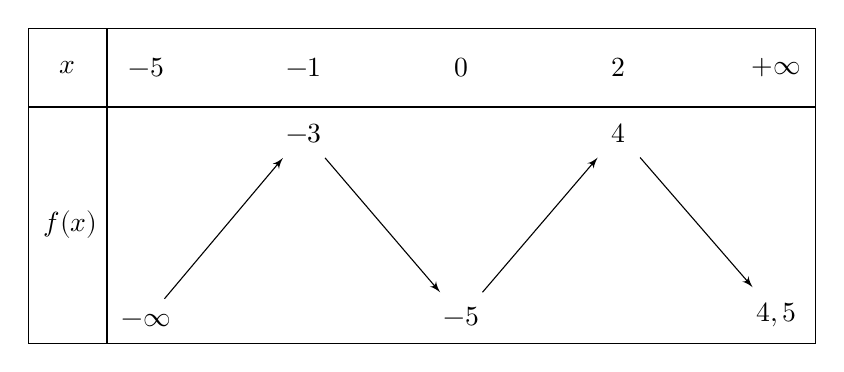
\begin{tikzpicture}
\tkzTabInit[lgt=1,espcl=2]{$x$/1,$f(x)$/3} {$-5$,$-1$,$0$,$2$,$+\infty$}
\tkzTabVar{-/$-\infty$ ,+/$-3$,-/$-5$,+/$4$,-/${4,5}$}%
\end{tikzpicture}
\end{center}
Αν  $C_f$ είναι η γραφική παράσταση της $f$.}
\AQquestion{Η εξίσωση $f(x) = -2$ δέχεται στο διάστημα $(-5,\,+\infty)$}
{{μια μόνο λύση}, {δύο λύσεις},	{τέσσερις λύσεις}}
\end{alterqcm}	
\end{verbatim}
και θα πάρουμε 
\begin{center}
\includegraphics[scale=]{test2.pdf}
\end{center}



\subsubsection{Περιβάλλον \texttt{array}}

Ο πίνακας των ερωτήσεων-απαντήσεων δέχεται  και μαθηματικές εκφράσεις με περιβάλλον \texttt{array}. Ας δούμε το επόμενο παράδειγμα:\\
\begin{minipage}{0.4\linewidth}
\begin{verbatim}
\begin{alterqcm}[lq=5cm,symb=$\Box$]
\AQquestion{Το $(x,\,y)=(1,\,-1)$
είναι λύση του συστήματος: }
{{$ \left\lbrace
\begin{array}{ll}
2x + 3y &= 5 \\
x + y &=0
\end{array}\right.$},
{$ \left\{
\begin{array}{ll}
x + 4y &=-3 \\
2x + 3y &=-1
\end{array}\right.$},
{$ \left\lbrace
\begin{array}{ll}
\dfrac{x}{2}+\dfrac{y}{2} &=1\\
x - 2y &=3
\end{array}\right.$}
}
\end{alterqcm}
\end{verbatim}
\end{minipage}
\begin{minipage}{0.6\linewidth}
\includegraphics[scale=0.7]{array.pdf}	
\end{minipage}

\subsection{Ερωτήσεις πολλαπλής επιλογής με εικόνες}
Το πακέτο μας δίνει τη δυνατότητα να τοποθετήσουμε ως προτάσεις επιλογής, εικόνες. Για παράδειγμα με τον παρακάτω κώδικα και τις αντίστοιχες εικόνες κατασκευάζουμε το επόμενο τεστ.

\begin{minipage}{0.4\linewidth}
	\begin{verbatim}
	\begin{alterqcm}[lq=6cm,sep]
	\AQquestion[pq=2 cm]{Ποιον από
	τους τρεις πίνακες ζωγράφισε ο
	\textbf{Paul Gaugin}\vfill}%
	{{\hfil\includegraphics[scale=0.10]
	{paint_4.jpg}\hfil},
	{\hfil\includegraphics[scale=0.10]
	{paint_1.jpg}\hfil},
	{\hfil\includegraphics[scale=0.10]
	{paint_3.jpg}\hfil}}
	\AQquestion[pq=0.5cm]{Ποιος από
	τους τρεις ζωγράφισε τον πίνακα;\\
	\hfil\includegraphics[height=2.5in]
	{paint_2.jpg}\hfil}%
	{{Van Gogh},{Pierre Renoir},
	{Paul C\'ezanne}}
	\end{alterqcm}
	\end{verbatim}
\end{minipage}
\begin{minipage}{0.6\linewidth}
	\includegraphics[scale=0.7]{paint.pdf}
\end{minipage}

\subsubsection{Test με ερωτήσεις Γεωμετρίας}
Ο πίνακας των ερωτήσεων - απαντήσεων δέχεται και γεωμετρικά σχήματα, είτε ως εικόνες με το geogebra ή άλλο πρόγραμμα, όπως δείξαμε παραπάνω είτε με απευθείας εισαγωγή με χρήση του πακέτου \textsf{tikz}. Ένα κλασσικό παράδειγμα βλέπουμε, τυπώνοντας τον παρακάτω κώδικα:
\begin{verbatim}
\begin{alterqcm}[lq=8cm,numprop=true,sep]
\AQquestion{Ανάμεσα στα διπλανά σχήματα ποιος είναι ο ρόμβος :}
{{\hspace{1cm} \begin{minipage}{5cm} 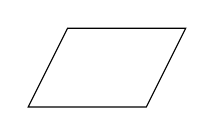
\begin{tikzpicture}
\draw (0,0)--(1.5,0)--(2,1)--(.5,1)--cycle;
\end{tikzpicture} \end{minipage}},
{\hspace{1cm} \begin{minipage}{5cm} 
\begin{tikzpicture}
\draw[rotate=30] (0,0) rectangle (1.5,1); \end{tikzpicture} \end{minipage}},
{\hspace{1cm} \begin{minipage}{5cm} 
\begin{tikzpicture}
\draw (0,0) rectangle (1,1); \end{tikzpicture} \end{minipage} }}
\end{alterqcm}
\nogreekalph 
\end{verbatim}
θα πάρουμε τον πίνακα 1
\begin{table}[h]
\includegraphics[scale=]{geometry.pdf}
\caption{}
\end{table}

\subsubsection{Πίνακας μεταβολών της $f$ και εξίσωση $f(x)=0$}
Γράφοντας τον κώδικα:
\begin{verbatim}
\begin{alterqcm}[lq=95mm,pre=false]
\AQmessage{ Έστω η συνάρτηση $f(x)=\sqrt{x(x-1)^2}$ ορισμένη στο διάστημα $[0,\,4]$ και
παραγωγίσιμη στο διάστημα $(0,\,1)\cup(1,4]$ της οποίας ο πίνακας μεταβολών δίνεται
παρακάτω:
\begin{center}
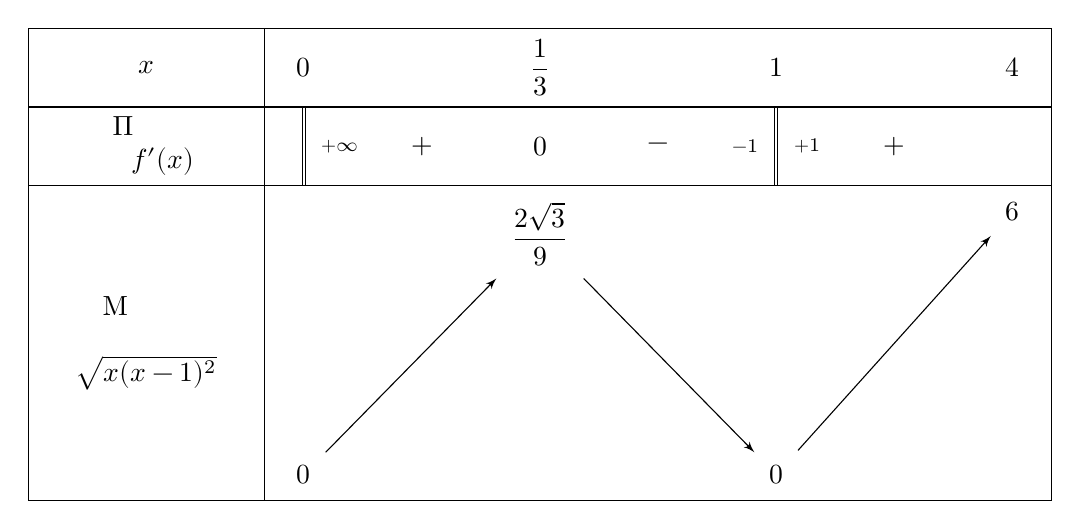
\begin{tikzpicture}
\tkzTabInit[lgt=3]%
{$x$/1,%
Πρόσημο\\ της $f^{\prime}(x)$ /1,%
Μεταβολές\\ της\\ $\sqrt {x(x-1)^2}$ /4}%
{$0$ , $\dfrac{1}{3}$ , $1$ , $4$}%
\tkzTabLine{d ,+, 0 ,-, d ,+, }
\tkzTabSlope{1//+\infty,3/-1 /+1}
\tkzTabVar{-/$0$,+/$\dfrac{2\sqrt3}{9}$,-/$0$,+/$6$}
\end{tikzpicture}
\end{center}
Αν  $C_f$ είναι η γραφική παράσταση της $f$.}
\AQquestion{Η εξίσωση $f(x) =1$ δέχεται στο διάστημα $(0,\,4)$}
{{μια μόνο λύση},
{δύο λύσεις},
{τρεις λύσεις},
{καμμία λύση}}
\end{alterqcm}	
\end{verbatim}
θα πάρουμε
\begin{center}
\includegraphics[scale=]{variationtable.pdf}
\end{center}

Για τις ασκήσεις με πίνακες μεταβολών καλό είναι να συμβουλευτείτε την ανάπτυξη του πακέτου στη διεύθυνση \texttt{https://tassosdimou.gr/variation-table}

\subsubsection{Ερωτήσεις πολλαπλής επιλογής και Σ-Λ στη Λογοτεχνία}
Ας δούμε ένα παράδειγμα με ερωτήσεις πολλαπλής επιλογής και σωστού-λάθους από τη Λογοτεχνία.

Γράφουμε τον κώδικα:
\begin{verbatim}
\begin{enumerate}
\item \begin{alterqcm}[lq=95mm,pre]
\AQquestion{Οι στίχοι:
\begin{verse}
<<Ο έρωτας\\
Το καράβι του\\
Κι η αμεριμνησία των μελτεμιών του\\
Κι ο φλόκος της ελπίδας του\\
Στον πιο ελαφρό κυματισμό του ένα νησί λικνίζει\\
Τον ερχομό.>>
\end{verse} γράφηκαν από τον:}
{{Σεφέρη},{Ελύτη},{Ρίτσο}}
\end{alterqcm}
\item \begin{alterqcm}[VF,lq=95mm,pre, title=false]
\AQquestion{Ο Οδυσσέας Ελύτης έγραψε τη
 <<Ρωμιοσύνη>>}
\AQquestion{ Ο Ηλίας Βενέζης έγραψε τη
 <<Γαλήνη>>}
\AQquestion{Ο Νίκος Καζαντζάκης έγραψε το
 <<Το αμάρτημα της μητρός μου>>}
\end{alterqcm}
\end{enumerate}
\end{verbatim}
και θα πάρουμε:
\begin{center}
\includegraphics[scale=0.8]{example_11_croped.pdf}
\end{center}

\subsubsection{Το \texttt{alterqcm} και η Φυσική}
Παρακάτω βλέπουμε την εφαρμογή του περιβάλλοντος \texttt{alterqcm} σε ένα τεστ Σωστού-Λάθους Φυσικής:
Ο κώδικας για το παρακάτω τεστ είναι:
\begin{verbatim}
\begin{alterqcm}[VF,lq=100mm,pre,long]
\AQquestion{Η συνισταμένη δυο δυνάμεων που ασκούνται σε
ένα σώμα είναι μηδέν ότα οι δυνάμεις έχουν το ίδιο μέτρο και αντίθετη φορά.}
\AQquestion{ Η δύναμη είναι μονόμετρο μέγεθος και στο S.I έχει μονάδα το 1N.}
.................................................
\AQquestion{Η δράση είναι μικρότερη από την αντίδραση.}
\AQquestion{Ο τρίτος νόμος του Νεύτωνα ισχύει σε όλες
τις περιπτώσεις.}
\end{alterqcm}
\end{verbatim} 
\begin{table}[!htp]
\includegraphics[scale=]{long1.pdf}
\caption{}
\end{table}

Ας δούμε ένα τεστ με ερωτήσεις πολλαπλής επιλογής. Θα πληκτρολογήσουμε: 
\begin{verbatim}
\begin{alterqcm}[pre,lq=7cm]
\AQquestion{Στο παρακάτω διάγραμμα ταχύτητας-χρόνου (u-t)
\begin{center}
\includegraphics[scale=0.7]{sxhma_1.png}
\end{center}}
{{Η κλίση της ευθείας ισούται με την αλγεβρική τιμή της επιτάχυνσης},
{Το εμβαδόν ισούται αριθμητικά με τη μετατόπιση},
{Η ευθεία δεν ξεκινά από την αρχή των αξόνων}}
...........................................
\AQquestion{Η καμπύλη του σχήματος αντιστοιχεί
 σε κίνηση:
\begin{center}\includegraphics[scale=0.8]{sxhma_2.png}
\end{center}}{{ευθύγραμμη και ομαλή.},{ευθύγραμμη ομαλά 
επιβραδυνόμενη.},{ ευθύγραμμη ομαλά 
επιταχυνόμενη.},{ με σταθερή ταχύτητα.}
} 
\end{alterqcm}
\end{verbatim}
 και θα πάρουμε 
\begin{center}
\includegraphics[scale=]{physics.pdf}
\end{center}




	
\end{document}